\chapter{Evaluation and Analysis}

In the first part of this section we briefly depict the nature of the data set used for evaluation of the models and discuss some specifics of the implementation. In the next part we present the results of our analysis.

\section{Data Set}

\todo{Add proper credit to the authors and developers of slepemapy.cz.}

For the analysis we used data from the online system for practicing geography\footnote{\url{http://www.slepemapy.cz}}~\cite{Papousek2014}. The data set contains more than 10~million answers from thousands of unique users~\cite{Papousek2015}. The data were filtered to contain only students with at least 50 answers and usually divided into 5 data sets, each containing at least 30 thousand answers. The answers of students who registered before the oldest question in the data set was answered were removed since it could temper with the results (considering we are interested primarily in models based on timing information).

\section{Toolchain}

The models were implemented in Python programming language. Experiments were performed in the Jupyter Notebook interactive environment\footnote{Jupyter Notebook is an open sourced web application for interactive computing, see~\url{https://jupyter.org/}}. Here is a list of the used libraries and modules:

\begin{itemize}
  \item SciPy, NumPy, Pandas
  \item Scikit-Learn
  \item Matplotlib
  \item NetworkX
\end{itemize}

\section{Response Time}

The response time of student to a question indicates how much well the item is learned. If the student answered quickly, almost automatically, it is very likely they either know the place very well or don't at all, depending on the correctness of their answer. On the other hand when the response is longer, the student is probably familiar with the item and might even recall the correct answer.

The Figure~\ref{fig-response-time} demonstrates the relationship between students' response time and the probability of recall. If the student's answer was suspiciously fast (response time is lower than 800 milliseconds), it usually means they guessed and don't know the correct answer. If the response time is between 1500 and 2000 milliseconds, it may indicate the student knows the place.

Note that some places are bigger on the map then other, i.e. a question requiring the student to choose Russia on the map has generally lower response time than a question requiring to choose Andorra.

\begin{figure}[htbp]
  \centering
  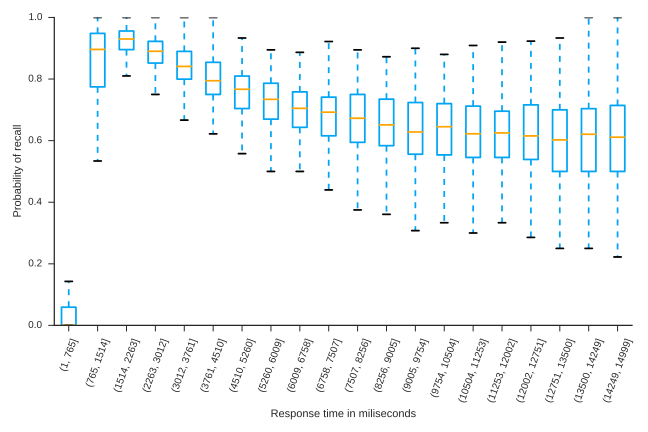
\includegraphics[width=\textwidth]{img/response-time}
  \caption{Relation between students' response time and probability of recall. Each box represents probabilities from all countries that belong in the relevant interval of response times.}
  \label{fig-response-time}
\end{figure}

\section{Calibration}

\section{Model Comparison}

\todo{The tables in this section aren't very readable, it should contain more information presented in a different way. Also it would be more interesting to adjust the parameters $\gamma$, $\delta$ for each data set.}
